\documentclass{beamer} 
% \usepackage{graphicx}
\usepackage{graphics}
\usepackage[T1]{fontenc}
\usepackage{verbatim}
\usepackage{etoolbox}
\usepackage{hyperref}
\usepackage{color}
\hypersetup{
  colorlinks   = true, %Colours links instead of ugly boxes
  urlcolor     = blue, %Colour for external hyperlinks
  linkcolor    = blue, %Colour of internal links
  citecolor   = red %Colour of citations
}
\makeatletter
\preto{\@verbatim}{\topsep=-6pt \partopsep=-6pt }
\makeatother
%\usepackage{fix-cm}
\setbeamercovered{transparent}


\renewcommand{\ni}{\noindent}


% \SweaveOpts{cache=TRUE, background="white"}


\title[ 2-Graphics]{2 - Advanced Graphics}
\subtitle{05 - Perception}
\date{\hspace{1in}}
\institute[ISU]{Iowa State University}

\begin{document}


\begin{frame}
\maketitle
\end{frame}


\begin{frame}
    \frametitle{Cost of an Education}
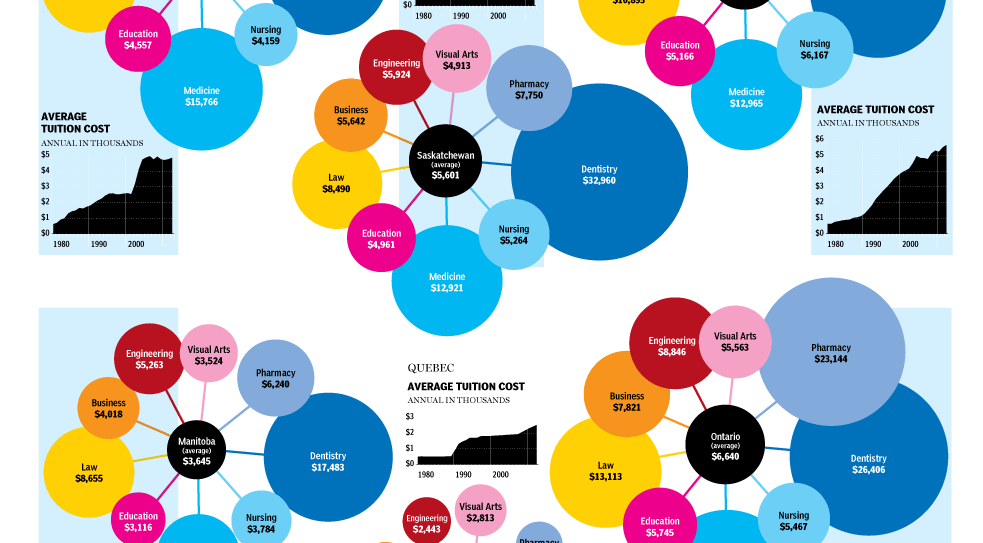
\includegraphics[keepaspectratio=TRUE,width=.9\linewidth]{junkcharts.png}
\end{frame}
\begin{frame}
    \frametitle{Motivation}
    \begin{itemize}
    \item Why are some plots easier to read?
    \hspace{-24pt}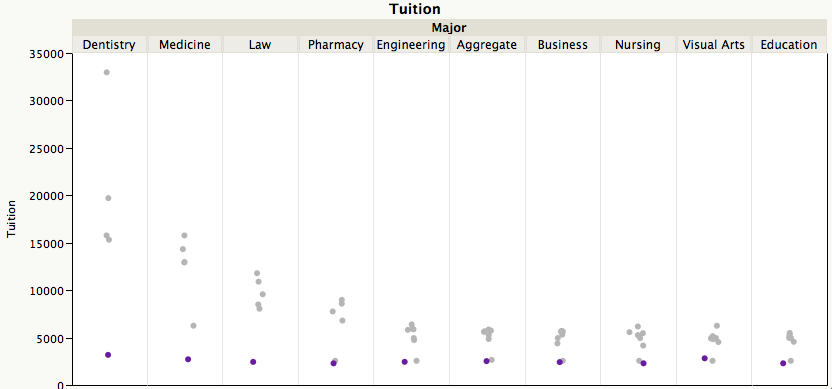
\includegraphics[keepaspectratio=TRUE,width=.9\linewidth]{dotplot.png}
    \item \url{http://junkcharts.typepad.com/junk_charts/2012/05/spring-flowers-and-striking-hours.html}
    \end{itemize}
\end{frame}

\begin{frame}
\frametitle{Good Graphics}
Graphics consist of 
\begin{itemize}
\item Structure (boxplot, scatterplot, etc.)
\item Aesthetics: features such as color, shape, and size that map other characteristics to structural features
\end{itemize}\bigskip
Both the structure and aesthetics should help viewers interpret the information.
\end{frame}

\begin{frame}
\frametitle{Outline}
\begin{itemize}
\item Cognitive aspects of perception and aesthetic choices\bigskip
\item Visual ordering mechanisms and color choices\bigskip
\item Faceting graphs to show additional variables\bigskip
\end{itemize}
\end{frame}


\begin{frame}
\frametitle{Pre-Attentive Features}
\begin{itemize}
\item Things that ``jump out" in less than 250 ms\medskip
\item Color, form, movement, spatial localization
\end{itemize}
\hfil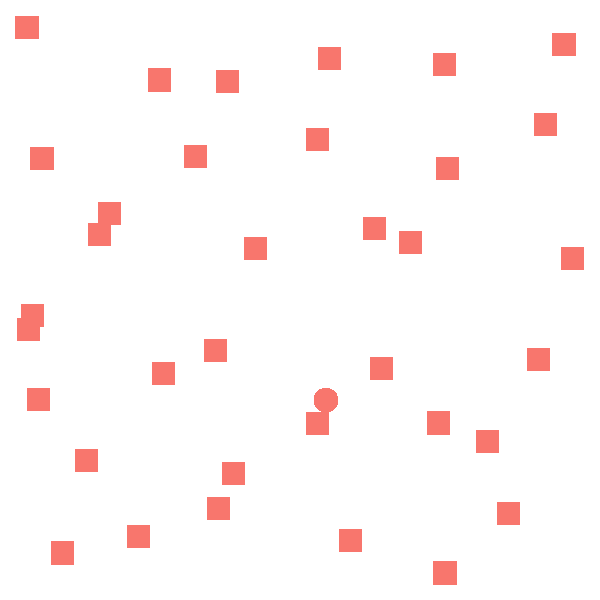
\includegraphics[width=.4\linewidth]{figure/preattentive11}\hspace{20pt}
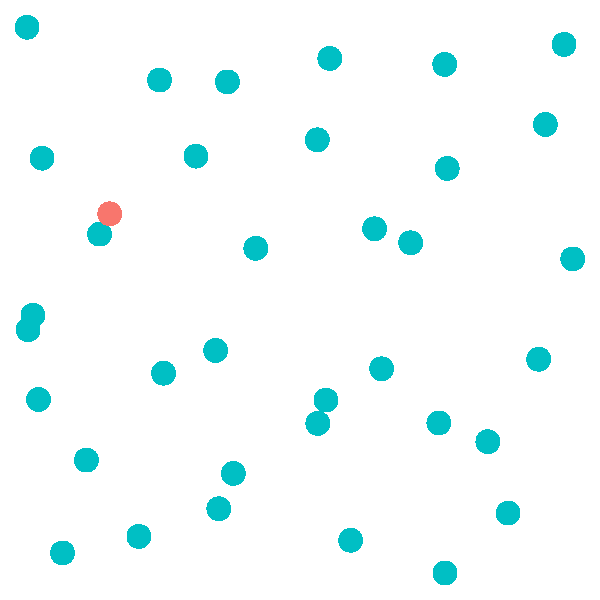
\includegraphics[width=.4\linewidth]{figure/preattentive12}
\end{frame}

% \begin{frame}
% \frametitle{Form}
% \begin{itemize}
% \item Size
% \item Angle
% \item Width
% \item Curvature
% \item Shape
% \item Length
% \item Grouping
% \item Added Marks
% \end{itemize}
% \end{frame}



\begin{frame}
\frametitle{Hierarchy of Features}
\begin{itemize}
\item Color is stronger than shape\medskip
\item Combinations of pre-attentive features are usually not pre-attentive due to \emph{interference}
\end{itemize}
\hfil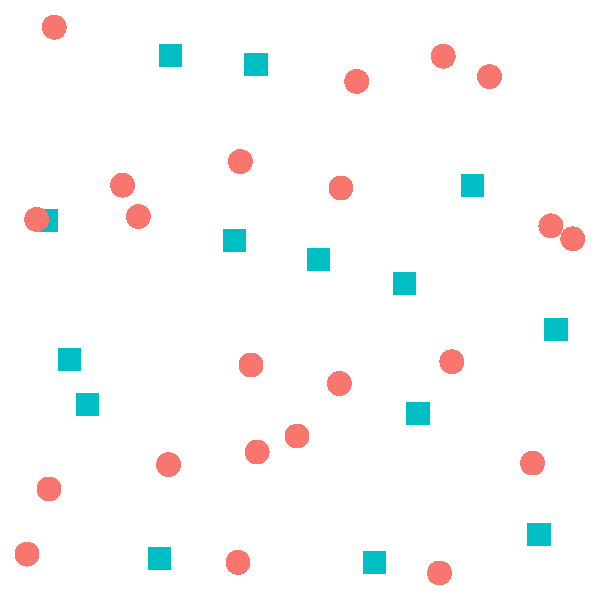
\includegraphics[width=.4\linewidth]{figure/preattentive21}\hspace{20pt}
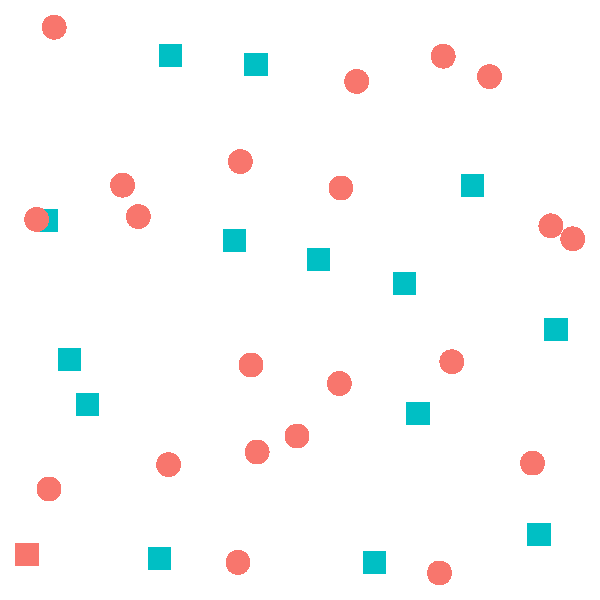
\includegraphics[width=.4\linewidth]{figure/preattentive22}
\end{frame}

\begin{frame}
\frametitle{Color}
\begin{itemize}
\item Hue: shade of color (red, orange, yellow...)
\item Intensity: amount of color
\item Both color and hue are pre-attentive. Bigger contrast corresponds to faster detection.
\end{itemize}
\begin{center}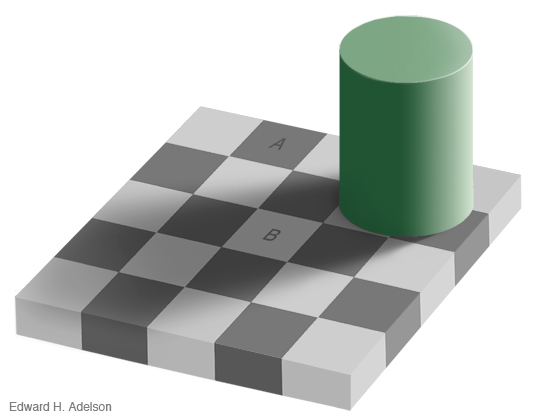
\includegraphics[keepaspectratio=TRUE,width=.3\textwidth]{shadowillusion}\end{center}
Color is context-sensitive: the exact same hue and intensity in one situation may appear to be a different color in a different context. A and B are the same intensity and hue, but appear to be different.
\end{frame}

\begin{frame}
\frametitle{Aesthetics in \texttt{ggplot2}}
\hfil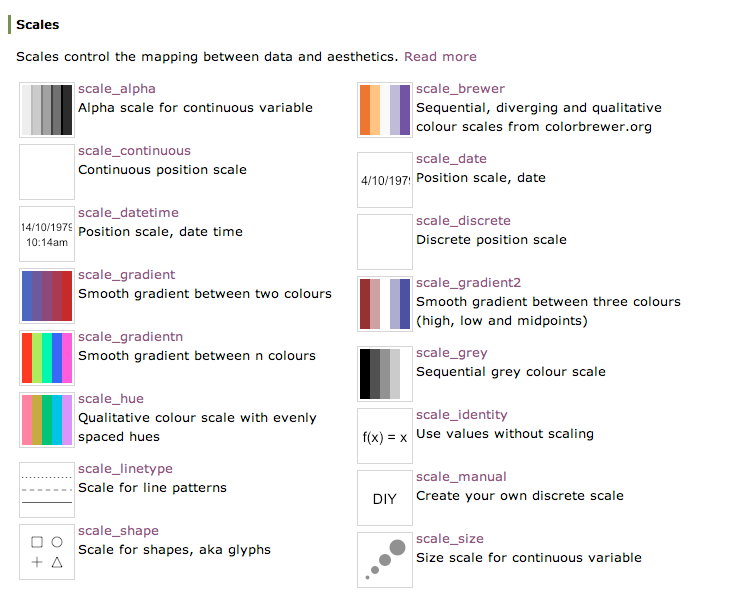
\includegraphics[width=.8\linewidth]{ggplot2aesthetics}\\
Main parameters: alpha, shape, color, size
\end{frame}

\begin{frame}[fragile]
\frametitle{Your Turn}
\vspace{-12pt}Find ways to improve the following graphic:















